\documentclass[a4paper, 14pt]{extarticle}

\usepackage{../generalPreamble}
\usepackage{../conspectFormat}
\usepackage{enumitem}

\begin{document}
\begin{titlepage}
    {\centering
        {\bfseries
            
\includegraphics[height=8cm]{../res/logo.jpeg}\\
            Unity. Precision. Perfection.\\
            \vspace{3.5cm}
            \uppercase{Конспект лекций} \\
            по дисциплине \enquote{Основы менеджмента качества и управления бизнес-процессами}\\
        }
        \vspace{\fill}
    }
    \begin{tabular}{l l}
        \textbf{Лектор}: & Рясков Ян Сергеевич\\
        \textbf{Страниц}: &\pageref{LastPage}\\
        \textbf{Последнее обновление}: & \today{}\\ 
        \textbf{Автор}: & Корытов Павел, 6304\\
    \end{tabular}

    \vspace{2cm}
    {\centering
        Санкт-Петербург \\
        \the\year\\
    }
\end{titlepage}

\tableofcontents
\newpage

\section{Качество: эволюция понятия}
\subsection{Основные стандарты менеджмента качества}
\begin{itemize}
    \item ГОСТ Р ИСО 9000–2015 --- ``Системы менеджмента качества, основные положения и словарь''. Разработан на основе стандарта ISO 9000. Описаны основные положения --- предназначение, принципы, основная терминология.
    \item ГОСТ Р ИСО 9001–2015 --- ``Системы менеджмента качества (СНК). Требования.'' Предназначен для сертификации.
    \item  ГОСТ Р ИСО 9004–2010 --- ``Менеджмент для достижения устойчивого успеха организации. Подход на основе менеджмента качества''
    \item  ГОСТ Р ИСО 19011–2012 --- ``Руководящие указания по аудиту системы менеджмента''
\end{itemize}

\subsection{Качество}
\dfn{Ценность товара} --- способность товара к удовлетворению ожиданий клиента.

\subsubsection*{Этапы развития качества}
\begin{enumerate}
    \item \dfn{Принцип мастерства} --- качество зависит от компетенции/квалификации группы лиц
    \item \dfn{Принцип У. Тейлора} --- Появление разделения труда, станков способствовало разработке границ допуска. Если детали выпускаются в этом интервале, продукт работает.\\
    Проблема, которая стоит до сих пор — сложность согласования границ.
    \item \dfn{Принципы Шухарта-Деминга} --- Методология статистического управления процессами и менеджмента качества. Использование статистических методов для снижения вариации.\\
    Любой продукт, который будет изготовлен по одной и той же спецификации, должен быть неотличим друг от друга. Таким образом, фокус смещается с конечного продукта на процессы производства
    \item \dfn{Принцип Тагути} --- Предложил использовать функцию от потерь и вариаций
\end{enumerate}

\begin{tcolorbox}
    \dfn{Качество} --- степень соответствия совокупности присущих характеристик объекта требованиям.
\end{tcolorbox}
\begin{itemize}
    \item Качество продукта
    \item Качество услуги
    \item Качество процесса
\end{itemize}

\dfn{Требования} — потребности или ожидания, которые установлены, обычно предполагаются или являются обязательными.

\dfn{Характеристика} --- некоторое отличительное свойство

\section{Система менеджмента}
\dfn{Система менеджмента (СМ)} --- это совокупность взаимосвязанных или взаимодействующих элементов организации для разработки политик, целей и процессов для достижения этих целей 

\dfn{Система мененджмента качества (СМК)} --- часть СМ, применительно к качеству.

\dfn{Процесс} --- совокупность взаимосвязанных и/или взаимодействующих видов деятельности, использующих входы для получения намеченного результата

\dfn{Потребитель} --- лицо или организация, которые могут получать или получают продукцию или услугу, предназначенные или требуемые этим лицом или организацией.

\subsection{Модель Кано}
\begin{figure}[h]
    \centering
    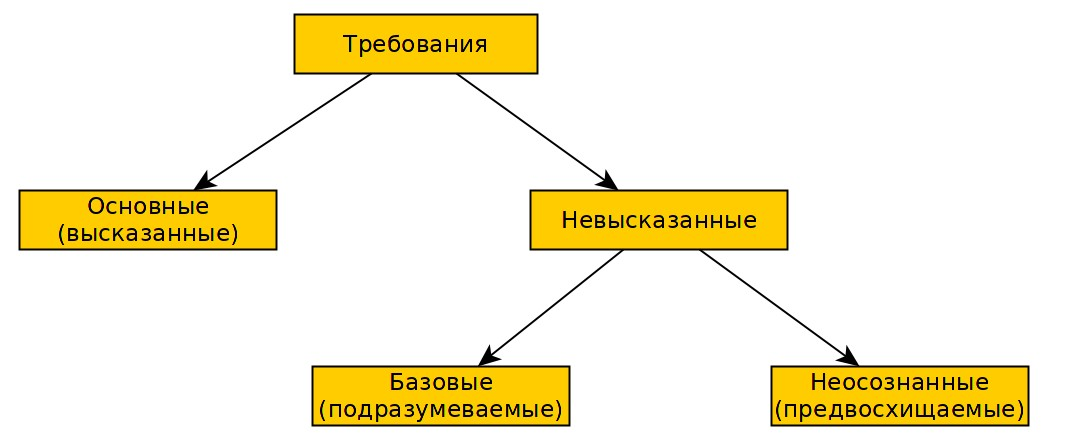
\includegraphics[width=0.8\textwidth]{./img/L2/S001.jpg}
    \caption{Классификация требований по Кано}%
    \label{img:l2:1}
\end{figure}

\dfn{Основные требования} --- те, которые напрямую влияют на потребителя. То, с чем товар выходит на рынок и ввязывается в конкурентную борьбу. Могут быть выявлены с помощью обычных маркетинговых исследований

\dfn{Базовые} --- требования по умолчанию. Сюда же относятся государственные стандарты. Эти требования сложно отследить в исследовании. Можно опросить клиентов о причине отказа от продукта.

\dfn{Неосознанные требования} --- некая ``фишка'' товара. Новшества, инновации и т.п.

\begin{figure}[h]
    \centering
    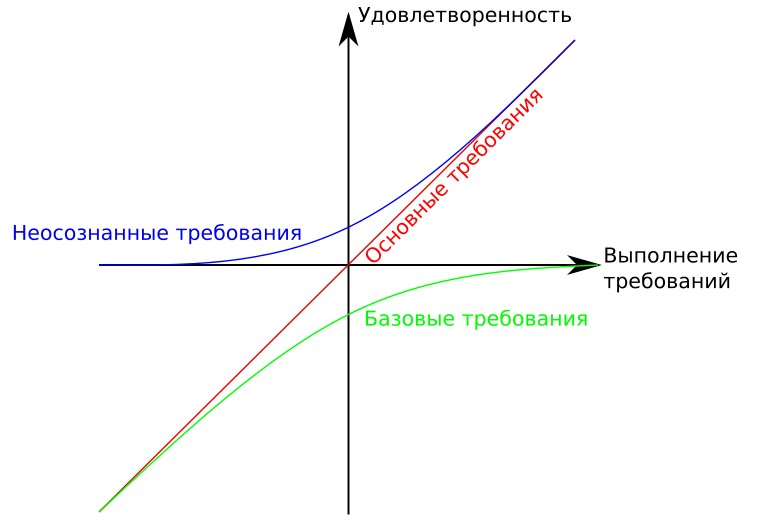
\includegraphics[width=0.7\textwidth]{./img/L2/S002.jpg}
    \caption{Удовлетворенность потребителя}%
    \label{img:l2:2}
\end{figure}

\dfn{Продукция} --- это выход организации, который может быть произведен без какого-либо взаимодействия между организацией и потребителем

\dfn{Услуга} --- выход организации с по крайней мере одним действием, обязательно осуществленным при взаимодействии организации и потребителя

\dfn{Характеристика качества} --- присущая характеристика продукции, процесса или системы, вытекающая из требований

\subsection{Операциональные определения}
Первыми работу в этом направлении начали Шухарт и Деминг.

\dfn{Операциональное определение} --- определение смысла на языке операций, с помощью которых он может быть проверен. Конкретизация значения того или иного термина применительно к конкретной системе и к конкретным людям, в ней задействованных, в зависимости от контекста. 

Элементы операционального определения:
\begin{itemize}
    \item \dfn{Критерий} --- стандарт, относительного которого оценивается результат тестов
    \begin{itemize}
        \item \dfn{Требование} --- Потребность или ожидание, которые установлено (задано), обычно предполагается или является обязательным
    \end{itemize}
    \item \dfn{Тест} --- метод испытания или процедура измерения свойства объекта
    \begin{itemize}
        \item \dfn{Испытание} --- Определение одной или нескольких характеристик, в соответствии с процедурой
    \end{itemize}
    \item \dfn{Решение} --- процедура принятия решения, показывает ли результат теста соответствие критерию
    \begin{itemize}
        \item \dfn{Анализ} --- Деятельность, предпринимаемая для определения пригодности, адекватности и результативности рассматриваемого объекта для достижения поставленных целей
        \item \dfn{Соответствие} --- Выполненное требование
        \item \dfn{Несоответствие} --- Невыполненное требование
    \end{itemize}
\end{itemize}

\subsubsection*{Соответствие характеристик требованиям}
\begin{figure}[h]
    \centering
    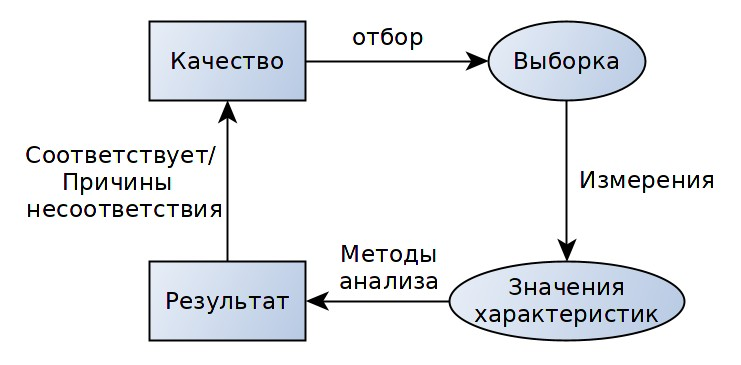
\includegraphics[width=0.6\textwidth]{./img/L3/S001.jpg}
\end{figure}

\subsection{Приницпы менеджмента качества}
\begin{enumerate}[label={\textbf{Принцип \arabic*.}}, align=left]
    \item Ориентация на потребителя
    \item Лидерство
    \item Вовлечение персонала
    \item Процессный подход
    \item Улучшение
    \item Принятие решений на основе фактических данных
    \item Управление взаимоотношениями
\end{enumerate}

\section{Анализ качества. Иструменты контроля}
В 1979 году Союз Японских Ученых и Инженеров выпустил ``7 основных иструментов контроля качества''. Основная задача --- предложить эффективный механизм потребления, не требующей особой математической подготовки

\subsection{Контрольный листок}
\dfn{Контрольный листок} --- бумажный бланк, используемый для сбора данных и их автоматического упорядочивания для облегчения дальнейшего использования собранной информации. Основное назначение --- представить информацию в удобном для обработки виде.

Должен отвечать следующим требованиям:
\begin{itemize}
    \item Удобен для заполнения
    \item Удобен для дальнейшего анализа собранных данных
\end{itemize}

\subsection{Гистограмма}
\dfn{Гистограмма} --- это инструмент, позволяющий зрительно оценить распределение статистических данных, сгруппированных по частоте попадания в заданный интервал.

Гистограмма применяется везде, где требуется проведение анализа точности и стабильности процесса для отслеживания показателей производства и наблюдения за качеством.

\subsection{Диаграмма Парето}
\dfn{Принцип Парето}, или \dfn{Принцип 80/20} правило, введенной социологом Вильфредом Парето: `` 20\% усилий принесут 80\% результата''

\begin{figure}[h]
    \centering
    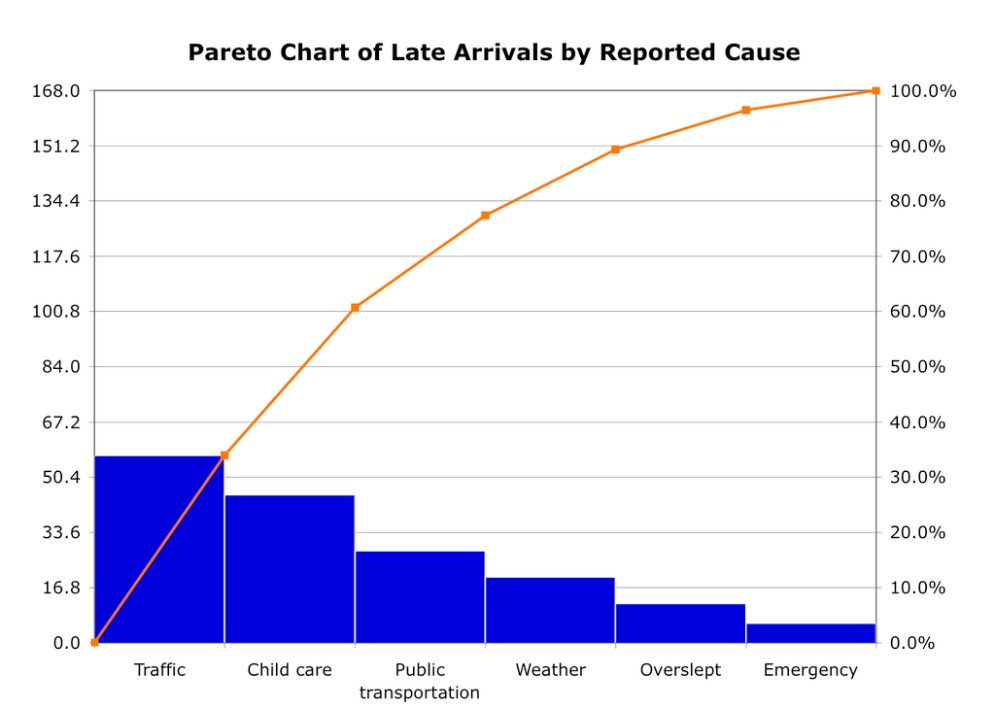
\includegraphics[width=0.8\textwidth]{./img/L4/S001.jpg}
    \caption{Пример диаграммы Парето}%
    \label{img:3:1}
\end{figure}

\dfn{Диаграмма Парето} --- графическое представление степени важности факторов
\begin{itemize}
    \item Определяет немногочисленные существенно важные причины проблемы
    \item Позволяет сэкономить ресурсы на устранение причин проблем
\end{itemize}

Типы диаграм Парето:
\begin{itemize}
    \item По результатам
    \item По причинам
\end{itemize}

\subsection{Диаграммы Исикавы}
\dfn{Диаграмма Исикавы}, \dfn{причинно-следственная диаграмма}, \dfn{диаграмма ``Рыбья кость''} --- инструмент, позволяющий выявить наиболее существенные факторы (причины), влияющие на конечный результат (следствие)

\begin{figure}[h]
    \centering
    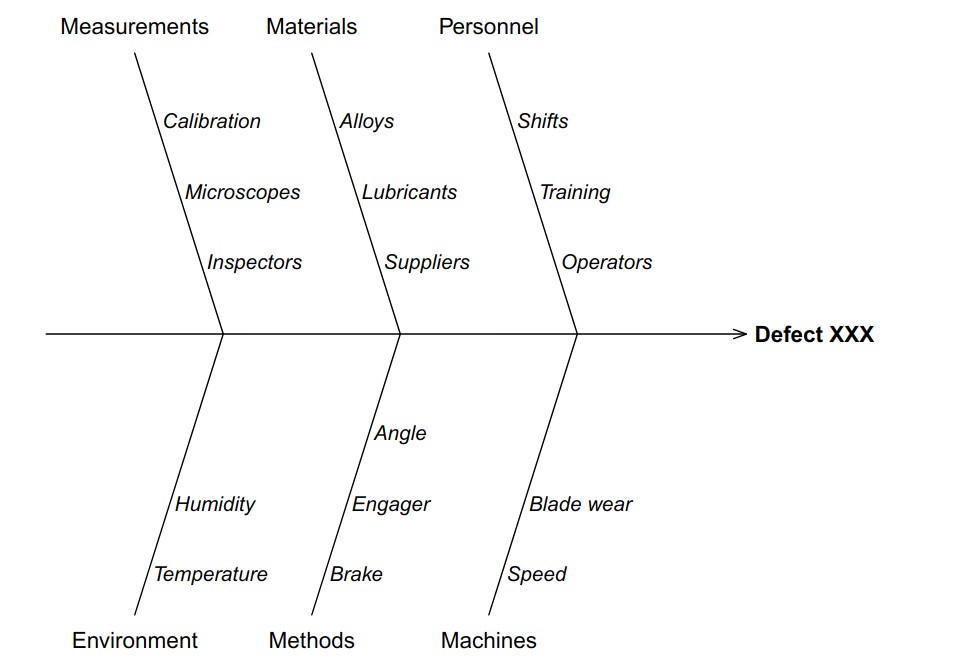
\includegraphics[width=0.5\textwidth]{./img/L4/S002.jpg}
    \caption{Пример диаграммы Исикавы}%
    \label{img:3:2}
\end{figure}

\subsection{Диаграмма рассеяния}
\dfn{Диаграмма рассеяния} --- это инструмент, позволяющий определить вид и тесносту связи двух рассматриваемых параметров процесса. 

\begin{figure}[h]
    \centering
    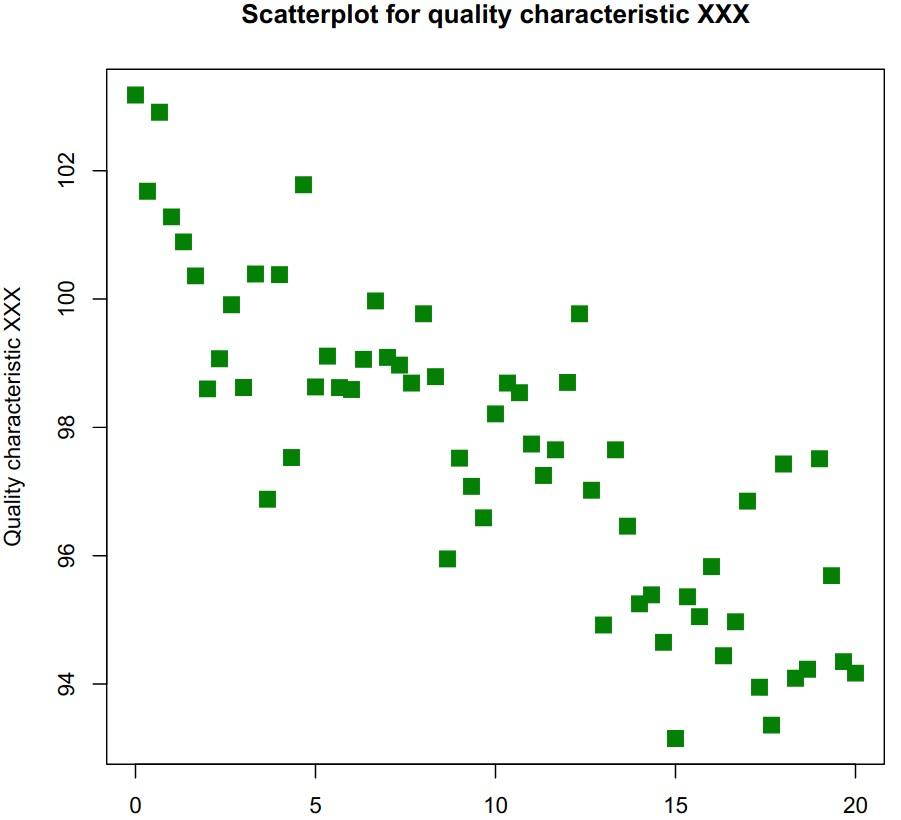
\includegraphics[width=0.6\textwidth]{./img/L4/S003.jpg}
    \caption{Пример диаграммы рассеяния}%
    \label{img:3:3}
\end{figure}

\subsection{Расслоение данных}
\dfn{Расслоение данных}, \dfn{стратификация} --- группировка данных по факторам

\subsection{Контрольные карты}
\dfn{Контрольная карта} --- графическое отображение состояния процесса, его уровня и изменчивости.

Цель --- обнаружить неестественные изменения в данных из повторяющихся процессов и дать критерии обнаружнния отсутствия статистической управляемости

\end{document}
